\documentclass[11pt,preprint]{elsarticle}

\usepackage{lmodern}
%%%% My spacing
\usepackage{setspace}
\setstretch{1.2}
\DeclareMathSizes{12}{14}{10}{10}

% Wrap around which gives all figures included the [H] command, or places it "here". This can be tedious to code in Rmarkdown.
\usepackage{float}
\let\origfigure\figure
\let\endorigfigure\endfigure
\renewenvironment{figure}[1][2] {
    \expandafter\origfigure\expandafter[H]
} {
    \endorigfigure
}

\let\origtable\table
\let\endorigtable\endtable
\renewenvironment{table}[1][2] {
    \expandafter\origtable\expandafter[H]
} {
    \endorigtable
}


\usepackage{ifxetex,ifluatex}
\usepackage{fixltx2e} % provides \textsubscript
\ifnum 0\ifxetex 1\fi\ifluatex 1\fi=0 % if pdftex
  \usepackage[T1]{fontenc}
  \usepackage[utf8]{inputenc}
\else % if luatex or xelatex
  \ifxetex
    \usepackage{mathspec}
    \usepackage{xltxtra,xunicode}
  \else
    \usepackage{fontspec}
  \fi
  \defaultfontfeatures{Mapping=tex-text,Scale=MatchLowercase}
  \newcommand{\euro}{€}
\fi

\usepackage{amssymb, amsmath, amsthm, amsfonts}

\def\bibsection{\section*{References}} %%% Make "References" appear before bibliography


\usepackage[numbers]{natbib}

\usepackage{longtable}
\usepackage[margin=2.3cm,bottom=2cm,top=2.5cm, includefoot]{geometry}
\usepackage{fancyhdr}
\usepackage[bottom, hang, flushmargin]{footmisc}
\usepackage{graphicx}
\numberwithin{equation}{section}
\numberwithin{figure}{section}
\numberwithin{table}{section}
\setlength{\parindent}{0cm}
\setlength{\parskip}{1.3ex plus 0.5ex minus 0.3ex}
\usepackage{textcomp}
\renewcommand{\headrulewidth}{0.2pt}
\renewcommand{\footrulewidth}{0.3pt}

\usepackage{array}
\newcolumntype{x}[1]{>{\centering\arraybackslash\hspace{0pt}}p{#1}}

%%%%  Remove the "preprint submitted to" part. Don't worry about this either, it just looks better without it:
\journal{Journal of Finance}

 \def\tightlist{} % This allows for subbullets!

\usepackage{hyperref}
\hypersetup{breaklinks=true,
            bookmarks=true,
            colorlinks=true,
            citecolor=blue,
            urlcolor=blue,
            linkcolor=blue,
            pdfborder={0 0 0}}


% The following packages allow huxtable to work:
\usepackage{siunitx}
\usepackage{multirow}
\usepackage{hhline}
\usepackage{calc}
\usepackage{tabularx}
\usepackage{booktabs}
\usepackage{caption}


\newenvironment{columns}[1][]{}{}

\newenvironment{column}[1]{\begin{minipage}{#1}\ignorespaces}{%
\end{minipage}
\ifhmode\unskip\fi
\aftergroup\useignorespacesandallpars}

\def\useignorespacesandallpars#1\ignorespaces\fi{%
#1\fi\ignorespacesandallpars}

\makeatletter
\def\ignorespacesandallpars{%
  \@ifnextchar\par
    {\expandafter\ignorespacesandallpars\@gobble}%
    {}%
}
\makeatother


% definitions for citeproc citations
\NewDocumentCommand\citeproctext{}{}
\NewDocumentCommand\citeproc{mm}{%
\href{\#cite.\detokenize{#1}}{#2}\nocite{#1}}

\makeatletter
% allow citations to break across lines
\let\@cite@ofmt\@firstofone
% avoid brackets around text for \cite:
\def\@biblabel#1{}
\def\@cite#1#2{{#1\if@tempswa , #2\fi}}
\makeatother
\newlength{\cslhangindent}
\setlength{\cslhangindent}{1.5em}
\newlength{\csllabelwidth}
\setlength{\csllabelwidth}{3em}
\newenvironment{CSLReferences}[2] % #1 hanging-indent, #2 entry-spacing
{\begin{list}{}{%
	\setlength{\itemindent}{0pt}
	\setlength{\leftmargin}{0pt}
	\setlength{\parsep}{0pt}
	% turn on hanging indent if param 1 is 1
	\ifodd #1
	\setlength{\leftmargin}{\cslhangindent}
	\setlength{\itemindent}{-1\cslhangindent}
	\fi
	% set entry spacing
	\setlength{\itemsep}{#2\baselineskip}}}
{\end{list}}

\usepackage{calc}
\newcommand{\CSLBlock}[1]{\hfill\break\parbox[t]{\linewidth}{\strut\ignorespaces#1\strut}}
\newcommand{\CSLLeftMargin}[1]{\parbox[t]{\csllabelwidth}{\strut#1\strut}}
\newcommand{\CSLRightInline}[1]{\parbox[t]{\linewidth - \csllabelwidth}{\strut#1\strut}}
\newcommand{\CSLIndent}[1]{\hspace{\cslhangindent}#1}


\urlstyle{same}  % don't use monospace font for urls
\setlength{\parindent}{0pt}
\setlength{\parskip}{6pt plus 2pt minus 1pt}
\setlength{\emergencystretch}{3em}  % prevent overfull lines
\setcounter{secnumdepth}{5}

%%% Use protect on footnotes to avoid problems with footnotes in titles
\let\rmarkdownfootnote\footnote%
\def\footnote{\protect\rmarkdownfootnote}
\IfFileExists{upquote.sty}{\usepackage{upquote}}{}

%%% Include extra packages specified by user

%%% Hard setting column skips for reports - this ensures greater consistency and control over the length settings in the document.
%% page layout
%% paragraphs
\setlength{\baselineskip}{12pt plus 0pt minus 0pt}
\setlength{\parskip}{12pt plus 0pt minus 0pt}
\setlength{\parindent}{0pt plus 0pt minus 0pt}
%% floats
\setlength{\floatsep}{12pt plus 0 pt minus 0pt}
\setlength{\textfloatsep}{20pt plus 0pt minus 0pt}
\setlength{\intextsep}{14pt plus 0pt minus 0pt}
\setlength{\dbltextfloatsep}{20pt plus 0pt minus 0pt}
\setlength{\dblfloatsep}{14pt plus 0pt minus 0pt}
%% maths
\setlength{\abovedisplayskip}{12pt plus 0pt minus 0pt}
\setlength{\belowdisplayskip}{12pt plus 0pt minus 0pt}
%% lists
\setlength{\topsep}{10pt plus 0pt minus 0pt}
\setlength{\partopsep}{3pt plus 0pt minus 0pt}
\setlength{\itemsep}{5pt plus 0pt minus 0pt}
\setlength{\labelsep}{8mm plus 0mm minus 0mm}
\setlength{\parsep}{\the\parskip}
\setlength{\listparindent}{\the\parindent}
%% verbatim
\setlength{\fboxsep}{5pt plus 0pt minus 0pt}



\begin{document}



%titlepage
\thispagestyle{empty}
\begin{center}
\begin{minipage}{0.75\linewidth}
    \centering
%Entry1
    {\uppercase{\huge Interest Rate Dynamics in South Africa: Evaluating
the South African Reserve Bank's Inflation Targeting Framework\par}}
    \vspace{2cm}
%Author's name
    {\LARGE \textbf{Tagishi Mashego}\par}
    \vspace{1cm}
%University logo
\begin{center}
    
\includegraphics[width=0.3\linewidth]{TexLogo.png}
\end{center}
\vspace{1cm}
%Supervisor's Details
\begin{center}
    {\Large \par}
    \vspace{1cm}
%Degree
    {\large \par}
    \vspace{1cm}
%Institution
    {\large Data Science For Economics and Finance 871\par}
    \vspace{1cm}
%Date
    {\large June 2025}
%More
    {\normalsize }
%More
    {\normalsize }
\end{center}
\end{minipage}
\end{center}
\clearpage


\begin{frontmatter}  %

\title{Interest Rate Dynamics in South Africa: Evaluating the South
African Reserve Bank's Inflation Targeting Framework}

% Set to FALSE if wanting to remove title (for submission)











\begin{abstract}
\small{
The stagflation experience of the 1970s and 1980s exposed significant
weaknesses in global financial systems, particularly in how monetary
economics is used to achieve macroeconomic objectives. The experience
played a pivotal role in central banks adopting the inflation-targeting
framework as the primary focus of their mandate. Since 2000, the South
African Reserve Bank has operated within a 3-6\% inflation target band.
Recently, the SARB has made clear its intention to move to a 3\% point
target, based on the view that lower inflation begets stronger economic
growth. Using the Global Macro dataset, this paper begins with a brief
assessment of the effectiveness of this framework, followed by an
empirical analysis of how this framework has influenced the behaviour of
short-term and long-term interest over time. The findings aim to give
valuable insight as to whether the SARB should proceed with this
proposed transition.
}
\end{abstract}

\vspace{1cm}


\begin{keyword}
\footnotesize{
Inflation targeting,~Interest Rates \\
\vspace{0.3cm}
}
\end{keyword}



\vspace{0.5cm}

\end{frontmatter}

\setcounter{footnote}{0}



%________________________
% Header and Footers
%%%%%%%%%%%%%%%%%%%%%%%%%%%%%%%%%
\pagestyle{fancy}
\chead{}
\rhead{}
\lfoot{}
\rfoot{\footnotesize Page \thepage}
\lhead{}
%\rfoot{\footnotesize Page \thepage } % "e.g. Page 2"
\cfoot{}

%\setlength\headheight{30pt}
%%%%%%%%%%%%%%%%%%%%%%%%%%%%%%%%%
%________________________

\headsep 35pt % So that header does not go over title




\section{\texorpdfstring{Introduction
\label{Introduction}}{Introduction }}\label{introduction}

The SARB has been given the constitutional mandate to protect the value
of the local currency. To achieve this mandate, it formally adopted the
inflation targeting framework in February 2000, with the explicit and
overarching aim to keep inflation low and stable. The measure of
inflation targeted at the time of adoption was the rate of change of the
overall consumer price index, excluding the mortgage interest cost
(CPIX) (\citeproc{ref-ellyne2011}{Ellyne \& Veller, 2011}). This target
changed to headline CPI inflation in 2009, following the alteration of
the measurement of housing costs, which essentially collapsed CPIX and
CPI into a single measure (\citeproc{ref-kahn2008}{Kahn, 2008}).

Under this framework, the SARB aims to keep inflation between 3-6\%,
with a preference closer to the midpoint of this band. The success of
this framework has been subject to much debate. According to Stiglitz
(\citeproc{ref-stiglitz2008}{2008}), inflation targeting is doomed to
inevitably fail, at great cost to those countries that maintain it. This
paper examines the validity of this statement by conducting an empirical
analysis to evaluate the behaviour of short-term and long-term interest
rates in South Africa since 2000, which, to a certain extent, serve as
indicators of conditions and monetary policy credibility. Finally, this
study gives insight into whether the SARB's pursuit of price stability
over this period justifies the transition to a 3\% point inflation
target.

\section{\texorpdfstring{Literature Review
\label{Literature Review}}{Literature Review }}\label{literature-review}

Globally, inflation targeting was first adopted in the 1990s, countries
like New Zealand and Canada were among the first to implement this
framework following the experience of stagflation, where a significant
portion of central banks accepted higher inflation in the hope that it
would boost economic growth, largely relying on the theoretical
foundations of the Phillips curve. However, this resulted in high
inflation and stagnant growth, exposing the shortcomings of this model,
particularly the failure to account for expectations
(\citeproc{ref-ellyne2011}{Ellyne \& Veller, 2011}). This would be a
turning point in monetary policy. Many countries, South Africa being
amongst them, explored several other ways of conducting monetary policy,
such as managing the exchange rates, which proved to be inferior to
inflation targeting (\citeproc{ref-loewald2025}{Loewald, Steinbach \&
Rakgalakane, 2025}). The late 1990s and early 2000s posted strong growth
and more stable inflation rates, with evidence suggesting that countries
that targeted inflation enjoyed, on average, 4.8\% less inflation over
the 1990-2004 period (\citeproc{ref-IMF2006}{International Monetary
Fund, 2006}).

Locally, there has been mixed reviews on the success of this framework,
studies show that since 2000, the SARB has missed its inflation target
in several years, not only prompting criticism from parties such as
COSATU ( Congress of South African Trade Unions ) but raising doubts
around how successful the regime has been in managing price stability,
relative to the previous regime (\citeproc{ref-ellyne2011}{Ellyne \&
Veller, 2011}). Unfortunately, these doubts have economic consequences.
If the SARB cannot credibly commit to staying within the band, then that
increases the perceived economic risk of lending into the economy,
especially given the dire state of our government. While short-term
rates are closely tied to the central bank's policy rate (the repo
rate), long-term rates are largely driven by inflation expectations and
the corresponding risk premium associated with long-term investments.
Both fundamentally depend on the credibility of the SARB's commitment to
its inflation mandate.

The inflation target band in South Africa is set jointly by the SARB and
the National Treasury. In the early years following the adoption of this
framework the inflation target band oscillated between a range of 3-5\%
and 3-6\%, since November 2003, it has remained constant at 3-6\%
(\citeproc{ref-ellyne2011}{Ellyne \& Veller, 2011}). However, the
empirical evidence suggests that this inflation range is an outlier
relative to comparable economies. Among the 149 emerging market and
developing economies with available data, South Africa's inflation rate
is ranked 94th as of 2024 (\citeproc{ref-loewald2025}{Loewald \emph{et
al.}, 2025}) . In response, the SARB has recently advocated for a
transition to an inflation point target of 3\%, scheduled for
implementation in 2027. The SARB argues that this point target is high
enough to avoid reaching the zero lower bound which still allows the
SARB reduce the lending rate to stimulate the economy. Further, the
target is considered high enough so that price frictions do not carry
economic costs when interest rates adjust, which support a more
effective monetary policy transmission
(\citeproc{ref-loewald2025}{Loewald \emph{et al.}, 2025}). This paper
adds to the literature by showing how interest rates have behaved since
the 2000 , providing insight into the credibility of the SARB and give
an idea of how economic agents might respond the transition to a lower
inflation target.

\section{\texorpdfstring{Data
Description\label{Data Description}}{Data Description}}\label{data-description}

This study uses the Global Macro Dataset, an open-source and regularly
updated database that compiles macroeconomic data for 243 countries. The
dataset integrates data from reputable international organizations, such
as the World Bank and the International Monetary Fund. The database
covers global macroeconomic trends from the early days of data
collection to projected estimates in 2030, with historical data compiled
by economic historians to ensure accuracy over time
(\citeproc{ref-muller2025}{Müller, Xu, Lehbib \& Chen, 2025}).

This study makes use of the inflation-related data for South Africa from
2000-2024, to examine insightful trends over this period.

\subsection{Analysis}\label{analysis}

\begin{figure}[H]

{\centering 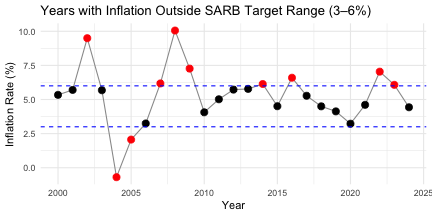
\includegraphics{DatSci-Project-_files/figure-latex/Figure1-1} 

}

\caption{Inflation Rates Since 2000 \label{Figure1}}\label{fig:Figure1}
\end{figure}

Figure \ref{Figure1} provides support for some of the criticisms
directed at the SARB. The SARB was unable to keep inflation within the
inflation target band in 10 of the years since 2000. An outlier occurred
in 2008 where the inflation rate reached 10.06\%, it is key to note that
this is before the Global Financial Crisis that would ensue, thus this
performance cannot be attributed to a once in a lifetime event, instead
oil price shocks and domestic price increases played a major role
(\citeproc{ref-honohan2022}{Honohan \& Orphanides, 2022}), indicating
that monetary policy failed to act aggressively enough to keep inflation
stable and within range.

\newpage

While consulting with additional other sources such as
(\citeproc{ref-StatsSA2004}{Statistics South Africa, 2004}) and
(\citeproc{ref-van2004}{Van der Merwe, 2004}), I have taken the -0.69\%
inflation rate in 2004 with a grain of salt because it does not fully
align with the literature, however, the consensus is that inflation in
this period was low and quite possibly lower than the 3\% bound, and yet
the South African economy saw strong growth, fueling belief that a lower
inflation rate is the key to growth.

The fact that the inflation rate reached 10.6\% in 2008 raised
significant concerns about the effectiveness of the inflation targeting
framework. Was it doomed to fail just as Stiglitz predicted? Since
economic agents base their investment decisions on their expectations of
the central bank's ability to achieve their commitment goal, the
credibility of the SARB is crucial. The next diagram uncovers how
interest rates have behaved following the 2008 peak, with the belief
that these interest rates represent agents' evolving perceptions of the
central bank's credibility.

\begin{figure}[H]

{\centering 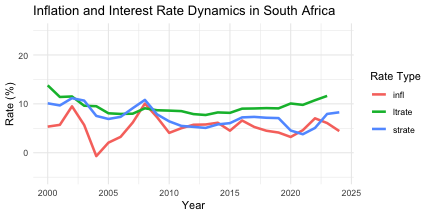
\includegraphics{DatSci-Project-_files/figure-latex/Figure2-1} 

}

\caption{ Behaviour of Market-Related Rates\label{Figure2}}\label{fig:Figure2}
\end{figure}

Following the inflation rate peak in 2008 as shown in \ref{Figure2} and
\ref{tab8}, long-term interest rates have consistently remained above
inflation and short-term interest rates. This suggests investors demand
higher returns for holding long-term investments, potentially reflecting
concerns about the riskiness of investing in South Africa and doubts
about the SARB's commitment to maintaining price stability.

The short-term interest rate has reacted ambiguously over this period.
This is not surprising because short-term interest rates typically track
the central bank rate (repo rate). Unless there is a complete loss of
credibility of the central bank, this rate will remain closely linked to
the central bank rate, as shown in below.

\begin{figure}[H]

{\centering 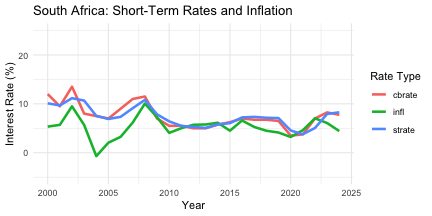
\includegraphics{DatSci-Project-_files/figure-latex/Figure3-1} 

}

\caption{Behvaiour of Short-Term Rates\label{Figure3}}\label{fig:Figure3}
\end{figure}

Figure \ref{Figure3} introduces the central bank rate to this paper,
commonly known as the repo rate in South Africa, which is the rate at
which the central bank lends to commercial banks. This is the primary
tool used by the SARB to influence short-term interest rates and
inflation. The repo rate is forward-looking, meaning that it is set
based on the central bank's expectation of future inflation. For
instance, should the SARB expect inflation to rise in the next year, it
may raise the repo rate now, even if current inflation is still within
the target. The figure shows that it is common practice for the central
bank to set the repo rate above inflation to maintain price stability.
However, during the 2021-2022 period, inflation exceeded the repo rate,
see \ref{tab9}. This deviation from normality can be largely attributed
to the COVID-19 pandemic, where economic activity had been limited since
2020, and the SARB kept the repo rate relatively fixed over this period
to help the economy recover.

\section{\texorpdfstring{Statistical
modelling\label{Statistical modelling}}{Statistical modelling}}\label{statistical-modelling}

To add rigour to the findings in Section \ref{Data Description} and to
capture the movements that may be lost in visual illustrations, this
section explores key econometric techniques to reinforce and validate
the findings.

As a precursor to the statistical modelling in this section, the
Autocorrelation function (ACF), Partial Autocorrelation function (PACF),
and Augmented Dickey Fuller (ADF) tests are conducted to test for the
stationarity of the variables. These diagnostic tests inform the
selection of the appropriate models for the variables of interest.

\subsection{Statistical Tests}\label{statistical-tests}

\subsubsection{Inflation}\label{inflation}

\begin{figure}[H]

{\centering 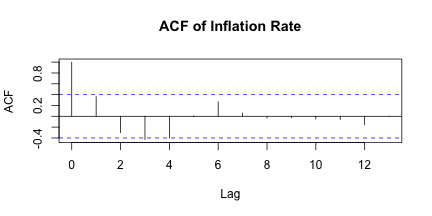
\includegraphics{DatSci-Project-_files/figure-latex/Figure10-1} 

}

\caption{Autocorrelation Function of Inflation \label{Figure10}}\label{fig:Figure10}
\end{figure}

\begin{figure}[H]

{\centering 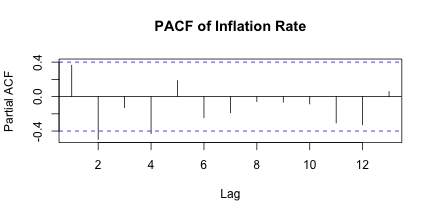
\includegraphics{DatSci-Project-_files/figure-latex/Figure11-1} 

}

\caption{Partial Autocorrelation Function of Inflation\label{Figure11}}\label{fig:Figure11}
\end{figure}

Figure \ref{Figure10} suggests a degree of inflation persistence, with
significant autocorrelation at the first and second lags. Whereas,
figure \ref{Figure11} suggests that there is a significant PACF at lag
1, this indicates that the first lagged period has a direct effect on
current inflation which usually means that a AR(1) model would be
sufficient, however based on the graph we cannot conclusively rule out
the possibility of a statistically significant second lag.

However, results for the ADF test rejects the null hypothesis of a unit
root, indicating that inflation is stationary. Based on this,
ARIMA(1,0,0) and ARIMA(2,0,0) models were estimated and compared.
ARIMA(2,0,0) model yielded the lowest values for both the Akaike
Information Criterion (AIC) and the Bayesian Information Criterion
(BIC), indicating that an AR(2) model is the most suitable for modeling
inflation.

\subsubsection{Short-Term Interest}\label{short-term-interest}

\begin{figure}[H]

{\centering 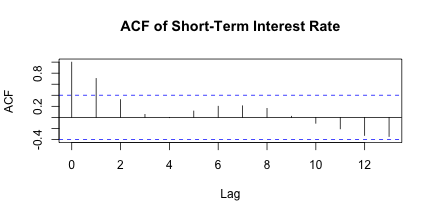
\includegraphics{DatSci-Project-_files/figure-latex/Figure12-1} 

}

\caption{Autocorrelation Function of Short-Term Interest Rate\label{Figure12}}\label{fig:Figure12}
\end{figure}

\begin{figure}[H]

{\centering 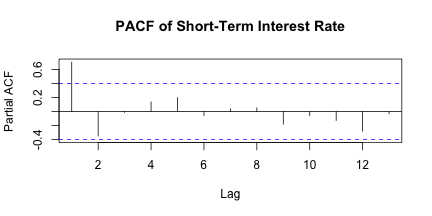
\includegraphics{DatSci-Project-_files/figure-latex/Figure13-1} 

}

\caption{ Partial Autocorrelation Function of Short-Term Interest Rate\label{Figure13}}\label{fig:Figure13}
\end{figure}

Figure \ref{Figure12} suggests a degree of short-term interest
persistence, with significant autocorrelation at the first, second and
third lags. Whereas, figure \ref{Figure13} suggests that there is a
significant PACF at lag 1, with an inconclusive second lag.

The results for the ADF test fails to reject the null hypothesis for a
unit root, indicating that short-term interest is non-stationary. After
taking the first difference this variable becomes stationary, indicating
that is I(1) and thus suitable for a VAR model.

\subsubsection{Long-Term Interest}\label{long-term-interest}

\begin{figure}[H]

{\centering 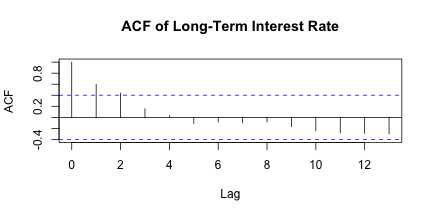
\includegraphics{DatSci-Project-_files/figure-latex/Figure14-1} 

}

\caption{Autocorrelation Function of Long-Term Interest Rate\label{Figure14}}\label{fig:Figure14}
\end{figure}

\begin{figure}[H]

{\centering 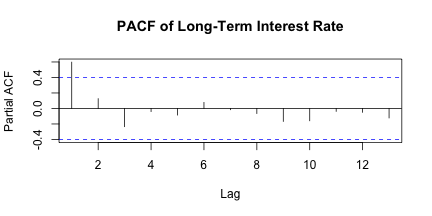
\includegraphics{DatSci-Project-_files/figure-latex/Figure15-1} 

}

\caption{Partial Autocorrelation Function of Long-Term Interest Rate\label{Figure15}}\label{fig:Figure15}
\end{figure}

Figure \ref{Figure14} suggests a degree of short-term interest
persistence, with significant autocorrelation at the first, second,
third and fourth lags. Whereas, figure \ref{Figure15} suggests that
there is a significant PACF at the first and second lags, with an
inconclusive third lag.

The results for the ADF test fails to reject the null hypothesis for a
unit root, indicating that long-term interest is non-stationary. The
long-term interest only became stationary after applying third
differencing, indicating it is I(3) and unsuitable for a VAR model.

\bigskip

\subsection{Modelling}\label{modelling}

The Autoregressive Model of order 2 for inflation is : \begin{equation}
\pi_t = c + \phi_1 \pi_{t-1} + \phi_2 \pi_{t-2} + \varepsilon_t
\end{equation}

\begin{table}[H]
\centering
\begin{tabular}{lrr}
  \hline
Term & Estimate & Std\_Error \\ 
  \hline
ar1 & 0.52 & 0.17 \\ 
  ar2 & -0.47 & 0.17 \\ 
  intercept & 5.25 & 0.38 \\ 
   \hline
\end{tabular}
\caption{AR(2) Model Coefficients for Inflation \label{tab66}} 
\end{table}

Table \ref{tab66} shows that a 1 unit increase in inflation in the first
lag increases current inflation by 0.524 units and that 1 unit increase
in inflation in the second lag decreases current inflation by 0.47
units. This suggests that inflation has short-term persistence but
ultimately reverts toward its long-run mean, which is about 5.25\%.

\bigskip

The following Vector Autoregressive Model (VAR(6)) was used to examine
the dynamic relationship between inflation and the short-term interest
rate:

\begin{equation}
\begin{bmatrix}
\pi_t \\
r_t
\end{bmatrix}
=
\mathbf{c}
+
\sum_{i=1}^{6}
\Phi_i
\begin{bmatrix}
\pi_{t-i} \\
r_{t-i}
\end{bmatrix}
+
\begin{bmatrix}
\varepsilon_{\pi,t} \\
\varepsilon_{r,t}
\end{bmatrix}
\end{equation}

\begin{table}[H]
\centering
\begin{tabular}{lrrr}
  \hline
Term & Estimate & Std\_Error & p\_value \\ 
  \hline
inflation.l1 & -0.03 & 0.51 & 0.95 \\ 
  short\_rate.l1 & 0.47 & 0.47 & 0.32 \\ 
  inflation.l2 & 0.03 & 0.50 & 0.95 \\ 
  short\_rate.l2 & -0.46 & 0.42 & 0.29 \\ 
  inflation.l3 & 0.24 & 0.33 & 0.46 \\ 
  short\_rate.l3 & -0.67 & 0.46 & 0.17 \\ 
  inflation.l4 & -0.73 & 0.33 & 0.10 \\ 
  short\_rate.l4 & 0.43 & 0.62 & 0.50 \\ 
  inflation.l5 & 0.70 & 0.43 & 0.14 \\ 
  short\_rate.l5 & -0.32 & 0.63 & 0.61 \\ 
  inflation.l6 & -0.23 & 0.42 & 0.60 \\ 
  short\_rate.l6 & -0.34 & 0.39 & 0.39 \\ 
  const & -0.32 & 5.03 & 0.95 \\ 
   \hline
\end{tabular}
\caption{VAR(6) Model Coefficient for the Short-Term Interest Rate \label{tab67}} 
\end{table}

The results shown in table \ref{tab67} indicate that none of the
coefficients are statistically significant at the 5\% level. However,
inflation at lag 4 shows marginal significance at the 10\% level.
Overall, these results suggest no evidence of statistically significant
interdependence between inflation and the short-term interest rate
within a six-period lag structure.

\section{Conclusion}\label{conclusion}

This paper assesses the credibility of the SARB under the
inflation-targeting regime to evaluate whether a transition to a lower
inflation target is both justified and likely to be perceived as
credible by economic agents. By analysing the behaviour of short-term
and long-term interest rates, the findings show that even though the
SARB has not always kept inflation within the target range, the
empirical models show that the SARB solves inflation with a bit of a
lag. Thus, it has maintained the trust the markets and economic agents.
Further, it is important to note that while there have been deviations
in the behaviour of interest rates, the findings show that these
fluctuations are a result of shocks exogenous to the SARB rather than
policy inconsistency. This implies that instances where the inflation
target was barely missed may reflect lagged adjustments and external
shocks rather than a loss of credibility.

\newpage

Governor Lesetja Kganyago, has on multiple occasions made the remark
that a highly inflationary economy is one that is `` anti-poor''. A
lower inflation has the potential to increase productive investment, as
a result of lost economic uncertainty. The spillover of this creates an
environment that is conducive for economic growth and job creation. This
paper provides valuable insight into how the interest rate dynamics
reflect institutional credibility of the SARB, the findings in this
paper therefore support the argument that a transition to a 3\% point
target is feasible and may yield desirable outcomes for the South
African economy.

\newpage

\section*{References}\label{references}
\addcontentsline{toc}{section}{References}

\phantomsection\label{refs}
\begin{CSLReferences}{1}{1}
\bibitem[\citeproctext]{ref-ellyne2011}
Ellyne, M. \& Veller, C. 2011. What is the SARB's inflation targeting
policy, and is it appropriate?

\bibitem[\citeproctext]{ref-honohan2022}
Honohan, P. \& Orphanides, A. 2022. \emph{Monetary policy in south
africa, 2007-21}. (2022/29). WIDER Working Paper.

\bibitem[\citeproctext]{ref-IMF2006}
International Monetary Fund. 2006. \emph{Inflation targeting and the
{IMF}}. International Monetary Fund.

\bibitem[\citeproctext]{ref-kahn2008}
Kahn, B. 2008. Challenges of inflation targeting for emerging-market
economies: The south african case. \emph{Challenges for Monetary
Policy-makers in Emerging Markets}.

\bibitem[\citeproctext]{ref-loewald2025}
Loewald, C., Steinbach, R. \& Rakgalakane, J. 2025. \emph{Less risk and
more reward revising south africas inflation target}.

\bibitem[\citeproctext]{ref-muller2025}
Müller, K., Xu, C., Lehbib, M. \& Chen, Z. 2025. The global macro
database: A new international macroeconomic dataset.

\bibitem[\citeproctext]{ref-StatsSA2004}
Statistics South Africa. 2004. \emph{Consumer price index (CPI):
Headline, november 2004}. Statistics South Africa.

\bibitem[\citeproctext]{ref-stiglitz2008}
Stiglitz, J.E. 2008. The failure of inflation targeting. \emph{Project
Syndicate}. 13.

\bibitem[\citeproctext]{ref-van2004}
Van der Merwe, E.J. 2004. \emph{Inflation targeting in south africa}.
South African Reserve Bank.

\end{CSLReferences}

\newpage

\section*{Appendix}\label{appendix}
\addcontentsline{toc}{section}{Appendix}

\begin{table}[H]
\centering
\begin{tabular}{ll}
  \hline
Variable & Description \\ 
  \hline
infl & Inflation rate (\%) \\ 
  strate & Short-term interest rate (\%) \\ 
  ltrate & Long-term interest rate (\%) \\ 
  cbrate & Central bank rate (repo rate, \%) \\ 
   \hline
\end{tabular}
\caption{Variable Descriptions\label{tab21}} 
\end{table}

\begin{table}[H]
\centering
\begin{tabular}{rr}
  \hline
Year & Inflation Rate (\%) \\ 
  \hline
2000 & 5.34 \\ 
  2001 & 5.70 \\ 
  2002 & 9.49 \\ 
  2003 & 5.68 \\ 
  2004 & -0.69 \\ 
  2005 & 2.06 \\ 
  2006 & 3.24 \\ 
  2007 & 6.18 \\ 
  2008 & 10.06 \\ 
  2009 & 7.26 \\ 
  2010 & 4.06 \\ 
  2011 & 5.02 \\ 
  2012 & 5.72 \\ 
  2013 & 5.78 \\ 
  2014 & 6.14 \\ 
  2015 & 4.51 \\ 
  2016 & 6.59 \\ 
  2017 & 5.27 \\ 
  2018 & 4.50 \\ 
  2019 & 4.13 \\ 
  2020 & 3.22 \\ 
  2021 & 4.61 \\ 
  2022 & 7.04 \\ 
  2023 & 6.07 \\ 
  2024 & 4.43 \\ 
   \hline
\end{tabular}
\caption{Annual Inflation Rate in South Africa (2000–2024) \label{tab8}} 
\end{table}

\begin{table}[H]
\centering
\begin{tabular}{rrr}
  \hline
Year & Inflation Rate (\%) & Repo Rate (\%) \\ 
  \hline
2010 & 4.06 & 5.50 \\ 
  2011 & 5.02 & 5.50 \\ 
  2012 & 5.72 & 5.00 \\ 
  2013 & 5.78 & 5.00 \\ 
  2014 & 6.14 & 5.75 \\ 
  2015 & 4.51 & 6.25 \\ 
  2016 & 6.59 & 7.00 \\ 
  2017 & 5.27 & 6.75 \\ 
  2018 & 4.50 & 6.75 \\ 
  2019 & 4.13 & 6.50 \\ 
  2020 & 3.22 & 3.50 \\ 
  2021 & 4.61 & 3.75 \\ 
  2022 & 7.04 & 7.00 \\ 
  2023 & 6.07 & 8.25 \\ 
  2024 & 4.43 & 7.75 \\ 
   \hline
\end{tabular}
\caption{Annual Inflation and Repo Rate in South Africa (2010–2024) \label{tab9}} 
\end{table}

\bibliography{Tex/ref}





\end{document}
